
\documentclass[border=10pt]{standalone}

% ----------------------------
\usepackage{tikz}
\usepackage{fancyhdr}

% ----------------------------
\usetikzlibrary{arrows,shapes,positioning,calc}
\tikzset{
  % Define standard arrow tip
  >=stealth',
  % Define style for boxes
  box/.style={
    rectangle,
    rounded corners,
    draw=black, very thick,
    text width=7.5em,
    minimum height=2em,
    text centered},
  % Define round style
  round/.style={
    ellipse, draw, thick,
    node distance=1cm,
    minimum height=5mm
  },
  % Define arrow style
  arrow/.style={
    ->,
    thick,
    shorten <=2pt,
    shorten >=2pt,},
  % line
  line/.style = {draw, -stealth', thick},
}

\def\circledarrow#1#2#3{ % #1 Style, #2 Center, #3 Radius
\draw[#1,->] (#2) +(80:#3) arc(80:-260:#3);
}


% ----------------------------
\begin{document}

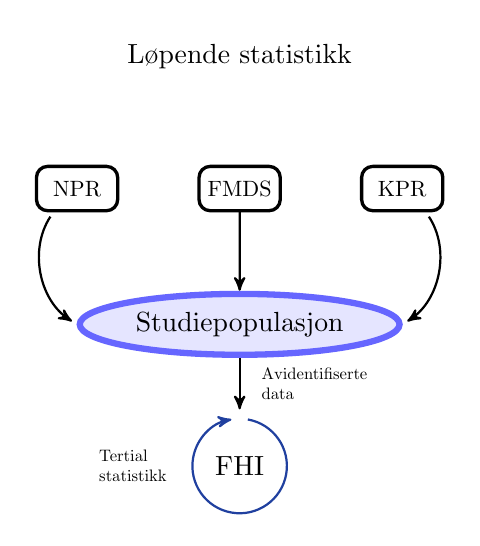
\begin{tikzpicture}[node distance=1cm, auto,]
  % nodes
  \node[box, text width=3em, scale=.8] (fmds) {FMDS};
  \node[box, draw=white, scale=1, text width=10em, above=of fmds] (title) {Løpende statistikk};
  \node[round, draw=blue!60, fill=blue!10, line width=0.8mm, below=of fmds] (population) {Studiepopulasjon};
  \node[box, draw=white, text width=4em, below=of population] (fhi){FHI};
  \node[box, text width=3em, scale=.8, right=of fmds] (kpr) {KPR}
     edge[arrow, bend left=45] (population.east);
  \node[box, text width=3em, scale=.8, left=of fmds] (NPR) {NPR}
     edge[arrow, bend right=45] (population.west);
  \path[line] (fmds) -- (population);
  \path[line] (population) -- node[right=.2, scale=.6, text width=3cm]
  {Avidentifiserte data}($(population)!.6!(fhi)$);
  \circledarrow{thick, draw={rgb:red,1;green,2;blue,5}}{fhi}{.6cm};
  \node[left=.01 of fhi, scale=.6, align=left] (t) {Tertial \\ statistikk};

\end{tikzpicture}
\end{document}
